\chapter{Short-Circuit Current in the Medium-Voltage Grid}
\label{chap:chapter2}
\index{short-circuit current}
\index{medium-voltage grid}
\index{transformer!parallel operation}

\section{General}
\label{sec:section21}

This example investigates the short-circuit current close to a substation when
two medium-voltage transformers, each rated at \SI{40}{\mega\volt\ampere}, are
operated in parallel. The transient simulation is compared with simple manual
estimates. The influence of an initial load and an additional short-circuit
reactor is then examined, followed by a steady-state AC analysis.

\section{Circuit Design}
\label{sec:section22}

We open the circuit-file \texttt{Shortcircuit\_Current.asc}. This example introduces the line device. Depending on the selected model, this device represents either an overhead line or an underground cable. Here, an oil-insulated underground cable with a conductor cross-section of \SI{500}{\milli\metre\squared} is assumed.

After placing the line element, we opened its attribute window by right-clicking the
symbol. We Double-clicked the \texttt{SpiceModel} field and selected the required
model. We deleted the attributes \texttt{Value2}, \texttt{SpiceLine}, and
\texttt{SpiceLine2}. In the \texttt{Value} attribute, we changed the length
parameter from 1 to 3, corresponding to a line length of \SI{3}{\kilo\metre}.

The high-voltage transformer uses the model
\texttt{RUYYo\_400k\_120k\_300MVA}. Its
\SI{400}{\kilo\volt} side is permanently grounded, whereas the
\SI{120}{\kilo\volt} side is isolated. The tap changer is set to \texttt{L+3}
using

\begin{lstlisting}[style=LTspice]
l_=3 (transformer tap value, pos. sign lower secondary voltage, neg. sign higher secondary voltage)
stproz=1.5 (percentage change in nominal voltage per tap step)
\end{lstlisting}

so that the secondary voltage is approximately \SI{116}{\kilo\volt}.

For the medium-voltage transformers, select the model
\texttt{RUYd5\_110k\_10k\_40MVA}. Their relative short-circuit voltage (ohmic part neglected) is set
to \SI{18}{\percent} with

\begin{lstlisting}[style=LTspice]
ux=0.18 (uk=sqrt(ux*ux+ur*ur))
\end{lstlisting}

The neutral points of the medium-voltage transformers on the \SI{110}{\kilo\volt} side are grounded through a Petersen coil, represented by the additional circuit element \texttt{pet}. The
two \SI{110}{\kilo\volt} lines are assumed to be compensated by this coil. One
cable produces an earth-fault current of approximately \SI{76}{\ampere}; 
This can be verified by deleting all the circuit elements after the line elements.
Now simulate the circuit \texttt{Shortcircuit\_Current.asc} and measure the peak current into the line by dividing the peak current by 1.414 and multiplying the result by three. The earth-fault current
can now be seen in the waveform viewer. % See also at ~\ref{ie:calculation} REFERENCE TO CALCULATION OF EARTH CURRENT   
The Petersen coil is rated at \SI{150}{\ampere} (\textasciitilde 2x76A) and is connected to both
transformer neutral points. When measuring the Petersen-coil voltage, you can observe a slowly varying amplitude during the settling process. This is because of the slight undercompensation or overcompensation of the Petersen coil

To obtain a realistic voltage across the Petersen coil, the phase-1
capacitance of line 1 is changed from \SI{400}{\nano\farad} to
\SI{401}{\nano\farad}. This introduces a small asymmetry. A Petersen coil is not modelled in this example on the \SI{10}{\kilo\volt} side. Because the transformer secondary
is delta-connected, a neutral point would be created with the grounding-transformer element
\texttt{Trafo\_gnd} element, connected to the transformer secondary terminals.

The earth-fault element \texttt{fault\_earth} is also introduced. It is
switched on at \SI{500}{\milli\second} by setting

\begin{lstlisting}[style=LTspice]
t_start=500m
\end{lstlisting}

\begin{remark}{Model asymmetry}{rem:remark21}
The deliberate \SI{1}{\nano\farad} capacitance difference prevents a perfectly
symmetrical zero-voltage condition across the Petersen coil.
\end{remark}

\section{Transient Simulation}
\label{sec:section23}

\subsection{Before the Fault}
The Petersen coil does not play a significant role in this short-circuit example.
We now start the simulation.
Before the fault, the line-to-line voltage is approximately
\SI{116}{\kilo\volt}and the line currents are predominantly capacitive charging
currents with a peak value of approximately \SI{35}{\ampere}.

\subsection{Fault Inception}
At fault inception, the short-circuit current at the fault position reaches a maximum instantaneous peak
value of approximately \SI{53}{\kilo\ampere}. The \SI{116}{\kilo\volt} voltage decreases to
approximately \SI{99}{\kilo\volt}. The RMS voltage can be checked at the measurement pins of bus4, the bus element on the right side

\begin{remark}{Output of measurement values}{rem:remark22}
The values calculated with .meas statements can be viewed in the SPICE output log. Activate the schematic window, select \texttt{View → SPICE Output Log}, and scroll to the end.
\end{remark}

\subsection{Settled Fault Current}
\label{sec:scc-simulation}
After the transient components have largely decayed---approximately
\SI{200}{\milli\second} after fault inception---the steady state short-circuit current is
approximately \SI{30}{\kilo\ampere} peak, or \SI{22}{\kilo\ampere} RMS. The
voltage on the \SI{400}{\kilo\volt} side is approximately
\SI{396}{\kilo\volt}.

\begin{result}{Transient simulation results}{result21}
The principal simulated values are a first peak of approximately
\SI{53}{\kilo\ampere} and a settled RMS short-circuit current of approximately
\SI{22}{\kilo\ampere}.
\end{result}

\section{Estimating the Steady-State Short-Circuit Current}
\label{sec:section24}

The RMS value of the steady-state short-circuit current can be estimated from
the transformer rating and relative short-circuit voltage. The rated current
on the medium-voltage side of one transformer is

\begin{calculation}{Short-circuit current estimate}{Calculation21}
\begin{align}
I_{N}
  &= \frac{S_N}{\sqrt{3}\,U_N} \\
  &= \frac{\SI{40}{\mega\volt\ampere}}
          {\sqrt{3}\cdot\SI{10.6}{\kilo\volt}} \\
  &\approx \SI{2.18}{\kilo\ampere}.
\end{align}

For a relative short-circuit voltage of $u_k=0.18$, the approximate
short-circuit-current factor is

\begin{equation}
\frac{1}{u_k}=\frac{1}{0.18}\approx 5.5.
\end{equation}

Thus, one transformer contributes approximately

\begin{equation}
I_{k,1}\approx 5.5\cdot\SI{2.18}{\kilo\ampere}
          =\SI{12}{\kilo\ampere}.
\end{equation}

For two identical transformers in parallel,

\begin{equation}
I_{k,2}\approx 2I_{k,1}=\SI{24}{\kilo\ampere}.
\end{equation}

This value applies at the nominal primary voltage of \SI{110}{\kilo\volt}.
Because the 110kV operating voltage decreases to approximately
\SI{100}{\kilo\volt}, the corrected estimate is

\begin{equation}
I_k\approx \frac{100}{110}\cdot\SI{24}{\kilo\ampere}
    =\boxed{\SI{21.8}{\kilo\ampere}}.
\end{equation}
\end{calculation}

Considering the simplifying assumptions, the manual estimate of approximately
\SI{21.8}{\kilo\ampere} agrees well with the simulated RMS value of
approximately \SI{22}{\kilo\ampere} in section \ref{sec:scc-simulation}.

\section{Short-Circuit Current with Initial Load}
\label{sec:section25}
Open the file \texttt{Shortcircuit\_Current\_with\_initial\_load.asc}.
A shunt reactor is used as the initial load. It reduces the operating voltage
and therefore also reduces the short-circuit current. The first current peak is
slightly lower, and the settled RMS current (Peak-value/1.414) is approximately
\SI{20.8}{\kilo\ampere}.

\section{Short-Circuit Reactor}
\label{sec:section26}
\index{short-circuit reactor}
Load file  \texttt{Shortcircuit\_Current\_with\_scr.asc}.
An additional short-circuit reactor, denoted by \texttt{scr} in the model, is
now introduced. For strongly inductive currents, its reactance causes a larger
voltage drop and limits the short-circuit current. During normal operation with
predominantly resistive current, the voltage drop across the reactor is much
smaller. The parameter \texttt{delta\_un=5\%} specifies the percentage voltage
drop at rated, purely inductive current.

With this reactor, the first transient current peak is reduced to approximately
\SI{11}{\kilo\ampere}, and the settled RMS short-circuit current is
approximately \SI{4.4}{\kilo\ampere}. The voltages are approximately
\SI{113.5}{\kilo\volt} on the \SI{110}{\kilo\volt} level,
\SI{399.8}{\kilo\volt} on the \SI{400}{\kilo\volt} level and
\SI{9}{\kilo\volt} on the \SI{10}{\kilo\volt} level.
\subsection{Manual Calculation}

For a reactor rated at $U_N=\SI{10}{\kilo\volt}$ and
$I_N=\SI{250}{\ampere}$ and with \texttt{delta\_un=5\%} , the nominal three-phase apparent power is

\begin{calculation}{Fault current behind the reactor}{calculation22}
\begin{align}
S_D
  &= \sqrt{3}\,U_N I_N \\
  &= \sqrt{3}\cdot\SI{10}{\kilo\volt}
     \cdot\SI{250}{\ampere} \\
  &\approx \SI{4.33}{\mega\volt\ampere}.
\end{align}

With the specified relative inductive voltage drop, the reactor impedance is

\begin{equation}
X_D=\frac{\Delta u_N}{100}\frac{U_N^2}{S_D}
   \approx\SI{1.15}{\ohm}.
\end{equation}

The maximum RMS fault current immediately behind the reactor is therefore

\begin{align}
I_{kD}
  &= \frac{U_N}{\sqrt{3}\,X_D} \\
  &= \frac{\SI{10}{\kilo\volt}}
          {\sqrt{3}\cdot\SI{1.15}{\ohm}} \\
  &\approx \SI{5}{\kilo\ampere}.
\end{align}

This assumes a perfectly stiff operating voltage. In the example, the voltage
drops from \SI{10.2}{\kilo\volt} to \SI{8.8}{\kilo\volt}; consequently, the
short-circuit current falls to approximately

\begin{equation}
	I_{kD}\approx\boxed{\SI{4.4}{\kilo\ampere}}.
\end{equation}
\end{calculation}

\section{AC Analysis}
\label{sec:scc-ac-analysis}
Load the file  \texttt{Shortcircuit\_Current\_AC.asc}. 
For the AC analysis, we first replaced the transient voltage-source model with the
corresponding AC source model. Then we adapted the \texttt{.meas} directives, deleted
the fault switch, and we placed the new ground element \texttt{ground} on the
schematic. We added the following option so that complex measurement results are
reported in polar form instead of decibels:

\begin{lstlisting}[style=LTspice]
.options meascplxfmt=polar
\end{lstlisting}

The magnitudes of the voltages and currents agree well with the settled values from
the transient analysis. Directly at the phaseA fault location, however, the
current angle is approximately \ang{120} rather than the initially expected
\ang{-90}. Closer to the voltage source---for example, at the transformer
primary side---the expected current angle of approximately \ang{-90} and voltage
angle of approximately \ang{0} are obtained.

\begin{important}{Effect of transformer vector group}{important21}
The transformer vector group is $\mathrm{Yd5}$, corresponding to a phase shift
of $5\cdot\ang{-30}=\ang{-150}$. For an almost purely inductive fault path, the
current lags the voltage by approximately \ang{-90}. Hence,
\begin{equation}
\varphi_I\approx\ang{-150}+(\ang{-90})=\ang{-240} = \ang{120}.
\end{equation}
Because the fault resistance is assumed to be purely resistive, the current
and the voltage at the fault have approximately the same angle. The theoretical
voltage angle can be checked by removing the ground elements and repeating the
simulation.
\end{important}

\begin{figure}[H]
	\centering
	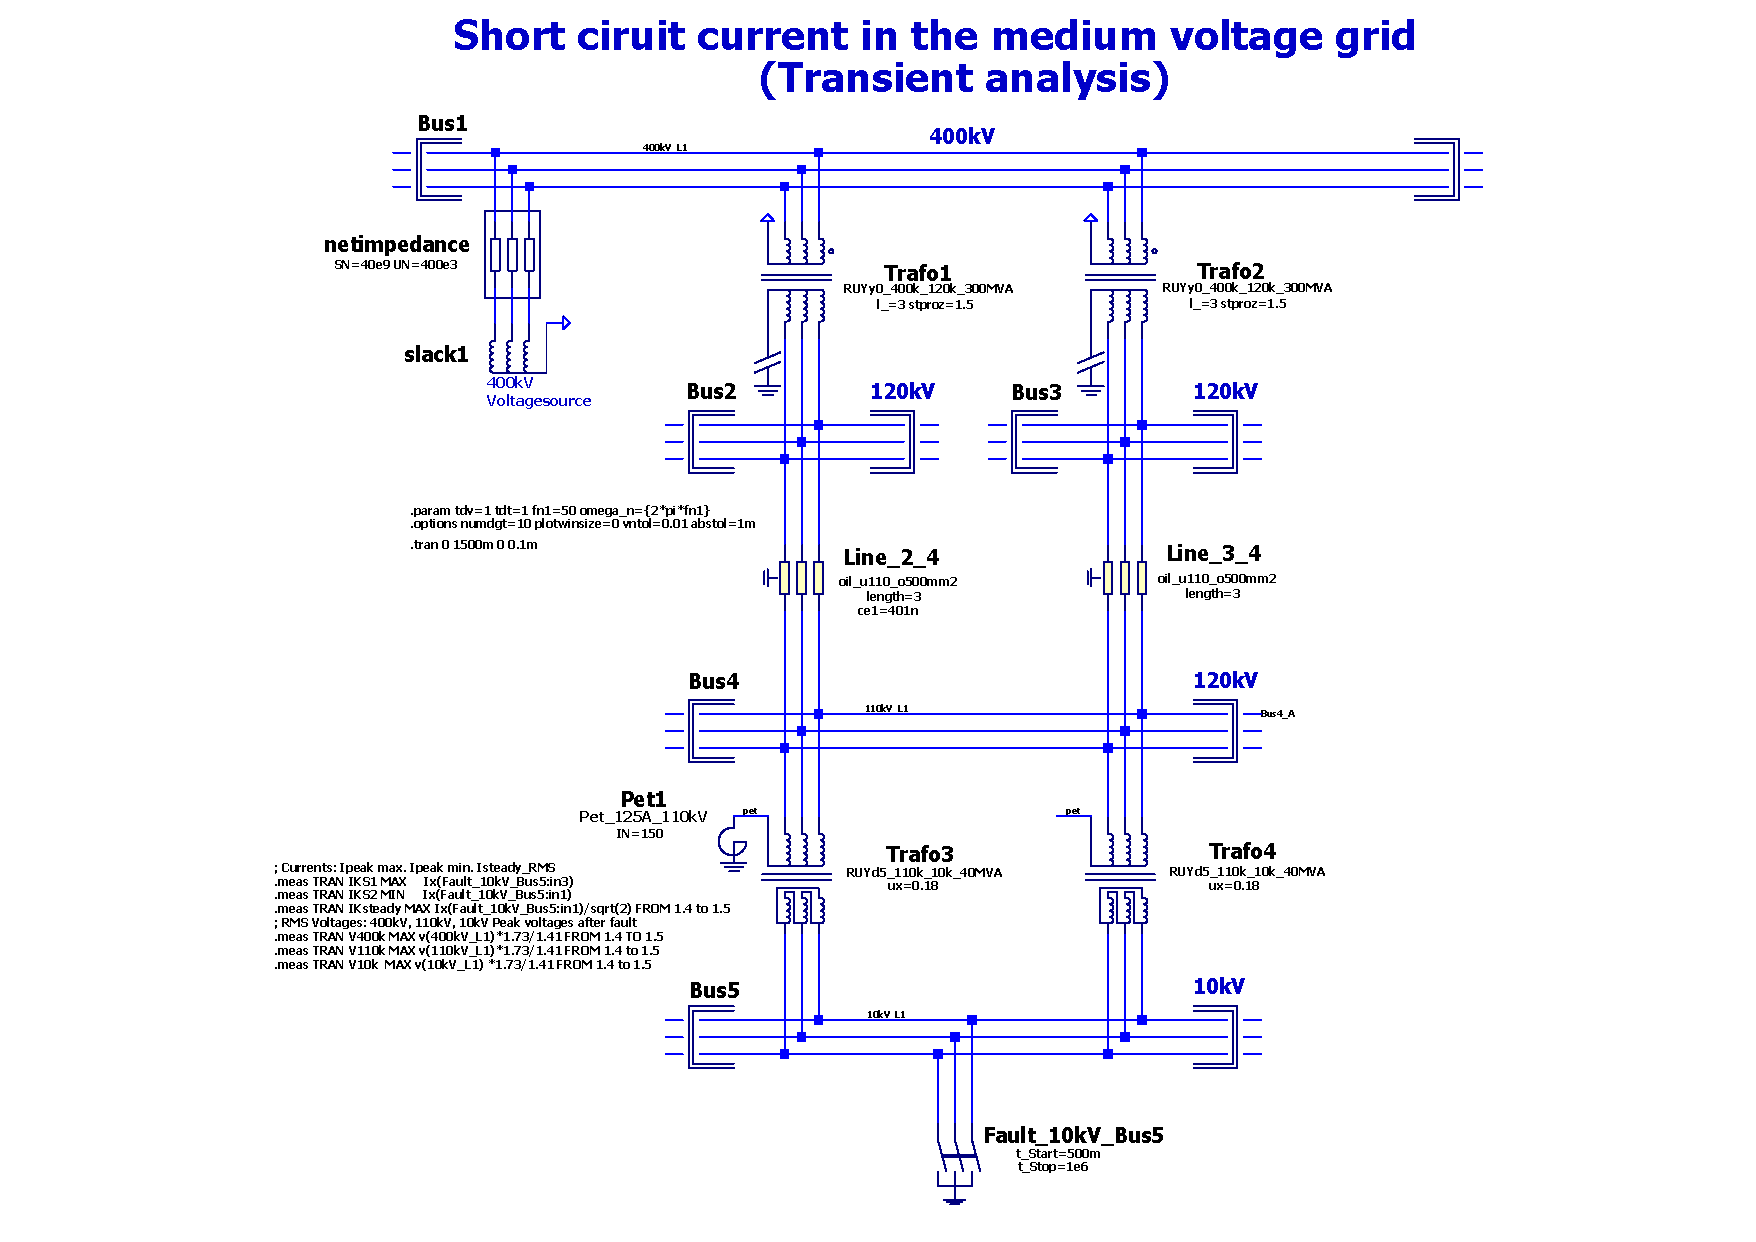
\includegraphics[width=1\textwidth] {figures/02_Shortcircuit in the medium voltage grid/Shortcircuit_Current_Schematic}
	\caption{Shortcircuit in the medium voltage grid - schematic}
	\label{fig:figure21}
\end{figure}

\begin{figure}[H]
	\centering
	\includegraphics[width=0.9\textwidth] {figures/02_Shortcircuit in the medium voltage grid/Shortcircuit_Current_Waveform}
	\caption{Shortcircuit in the medium voltage grid - waveform}
	\label{fig:figure22}
\end{figure}

\begin{figure}[H]
	\centering
	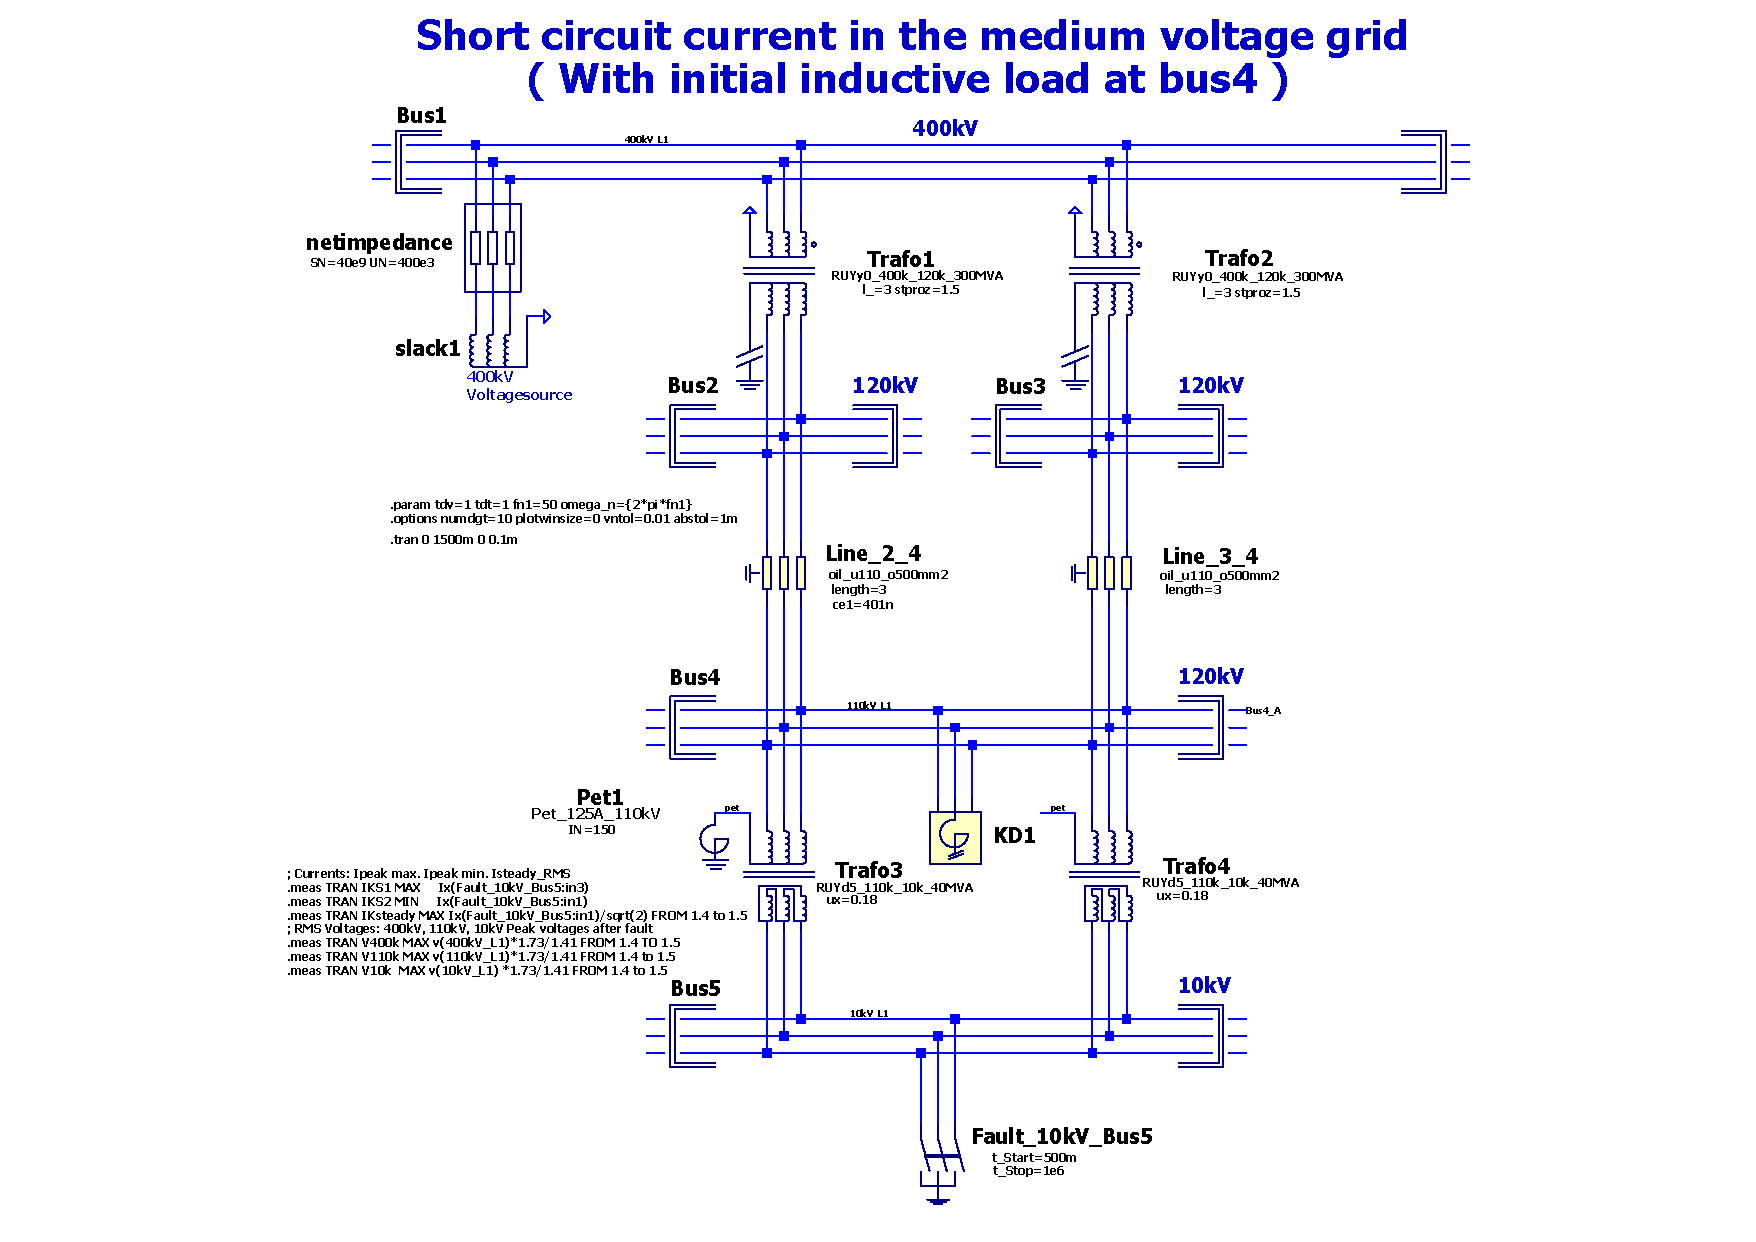
\includegraphics[width=1\textwidth] {figures/02_Shortcircuit in the medium voltage grid/Shortcircuit_Current_with_initial_load_schematic}
	\caption{Shortcircuit in the medium voltage grid with initial load - schematic}
	\label{fig:figure23}
\end{figure}

\begin{figure}[H]
	\centering
	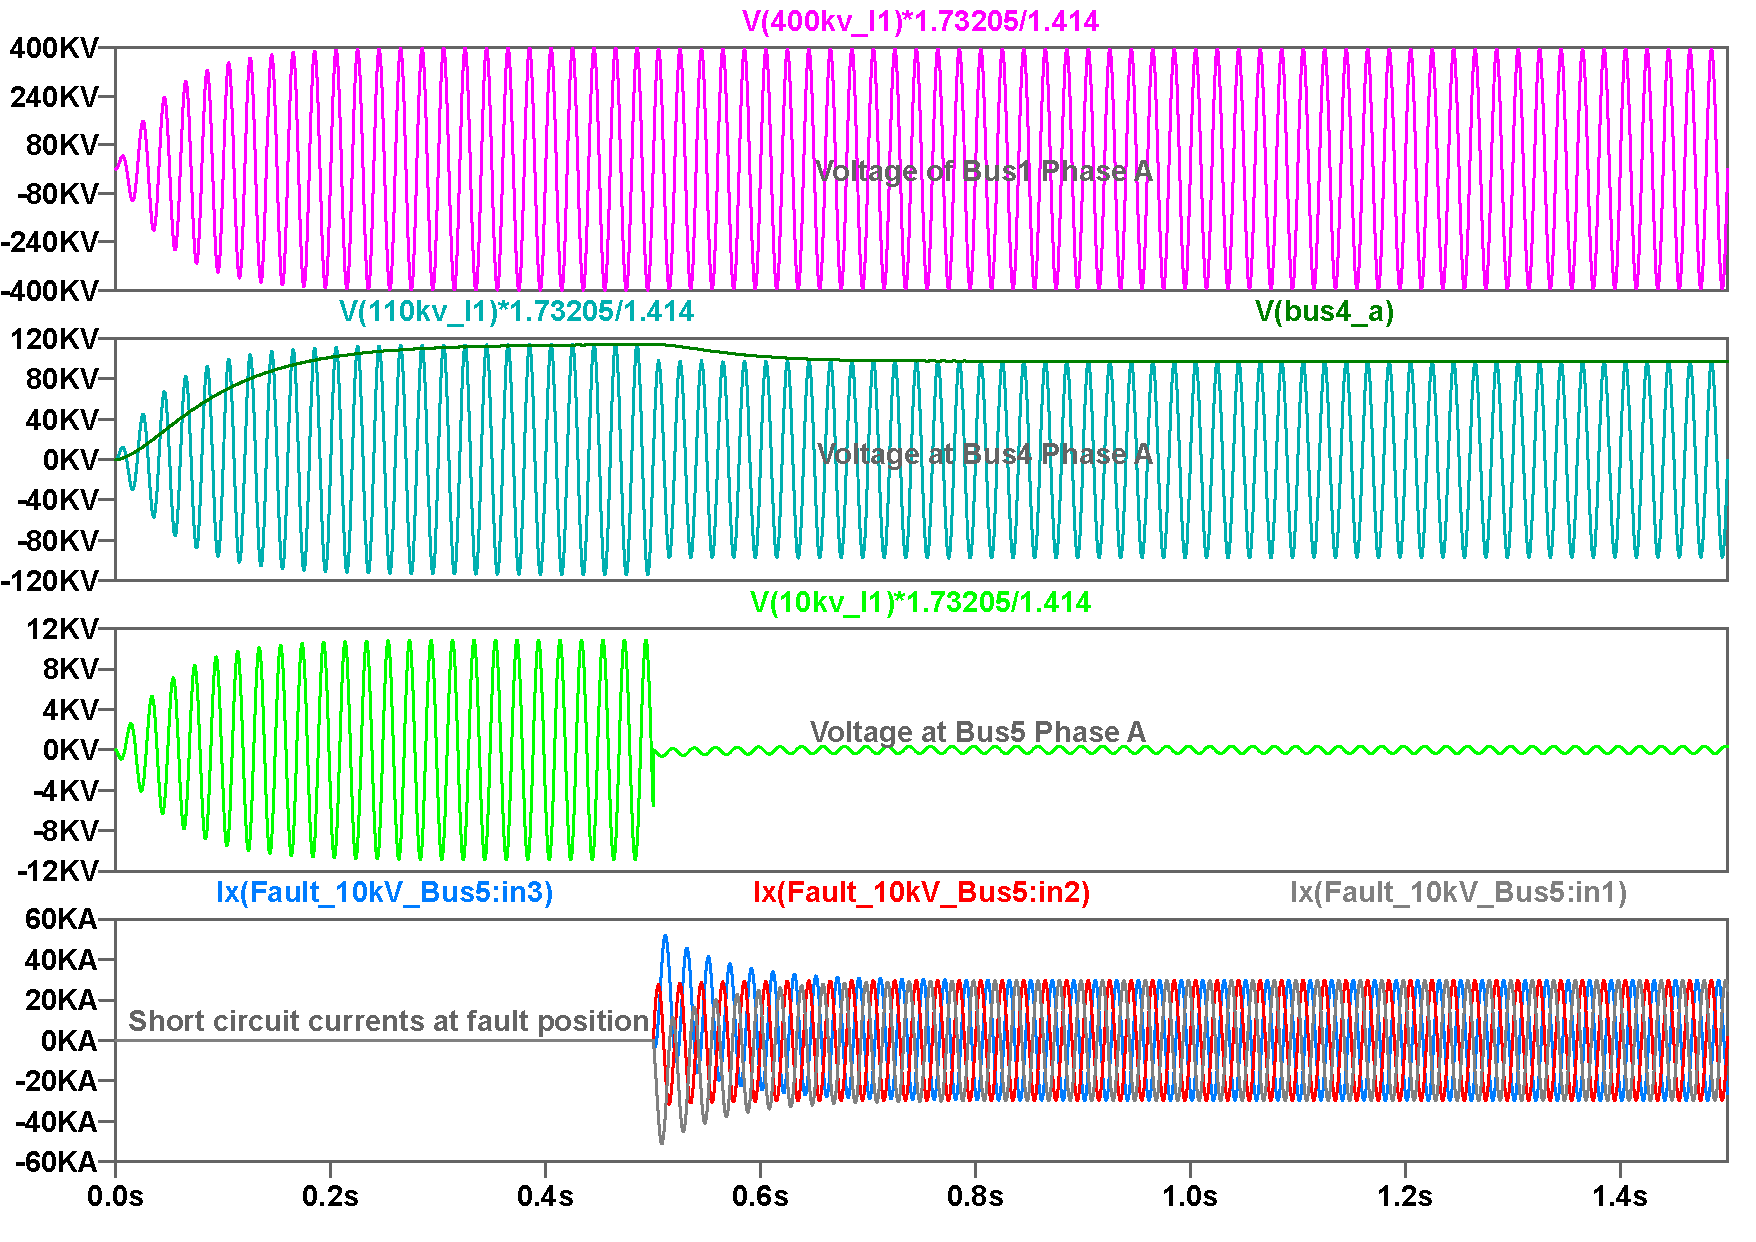
\includegraphics[width=0.9\textwidth] {figures/02_Shortcircuit in the medium voltage grid/Shortcircuit_Current_with_initial_load_waveform}
	\caption{Shortcircuit in the medium voltage grid with initial load - waveform}
	\label{fig:figure24}
\end{figure}

\begin{figure}[H]
	\centering
	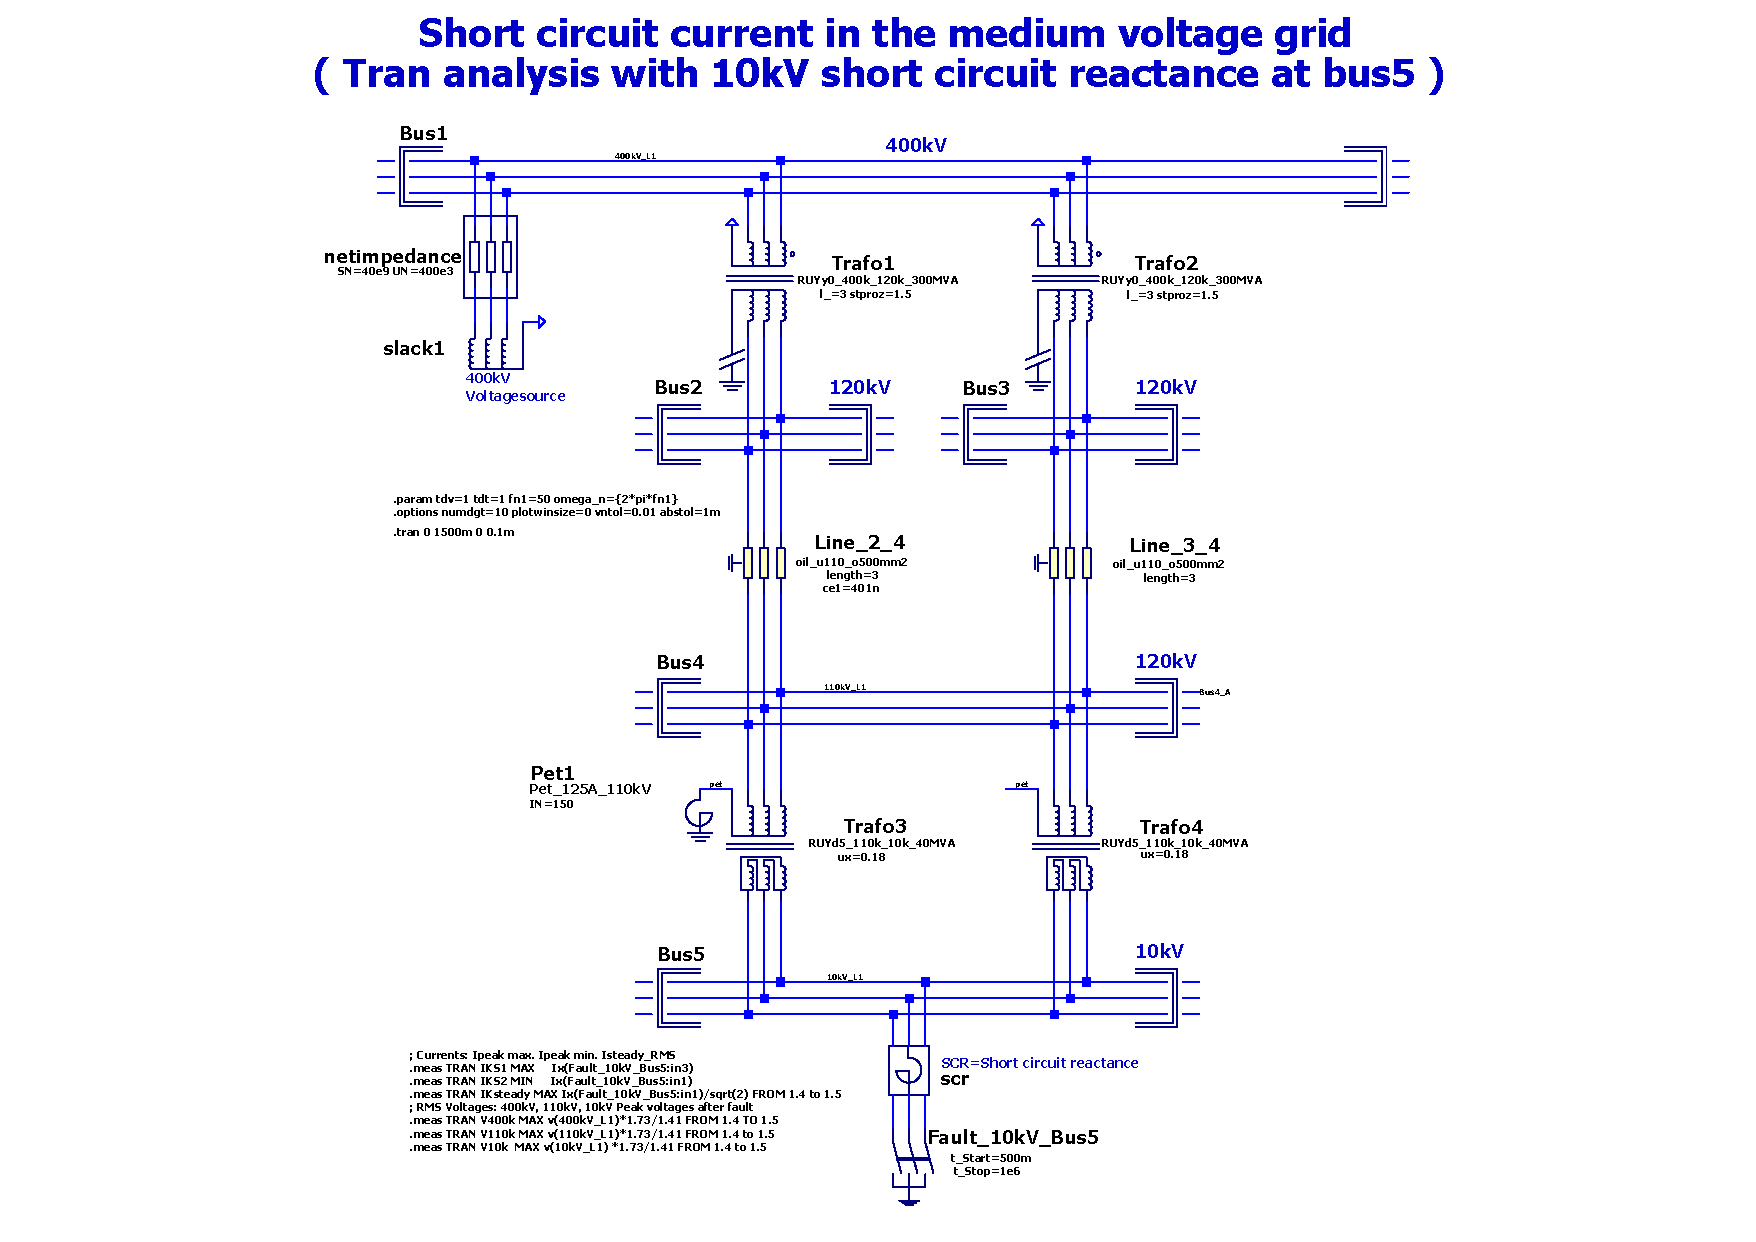
\includegraphics[width=1\textwidth] {figures/02_Shortcircuit in the medium voltage grid/Shortcircuit_Current_with_scr_schematic}
	\caption{Shortcircuit in the medium voltage grid with scr - schematic}
	\label{fig:figure25}
\end{figure}

\begin{figure}[H]
	\centering
	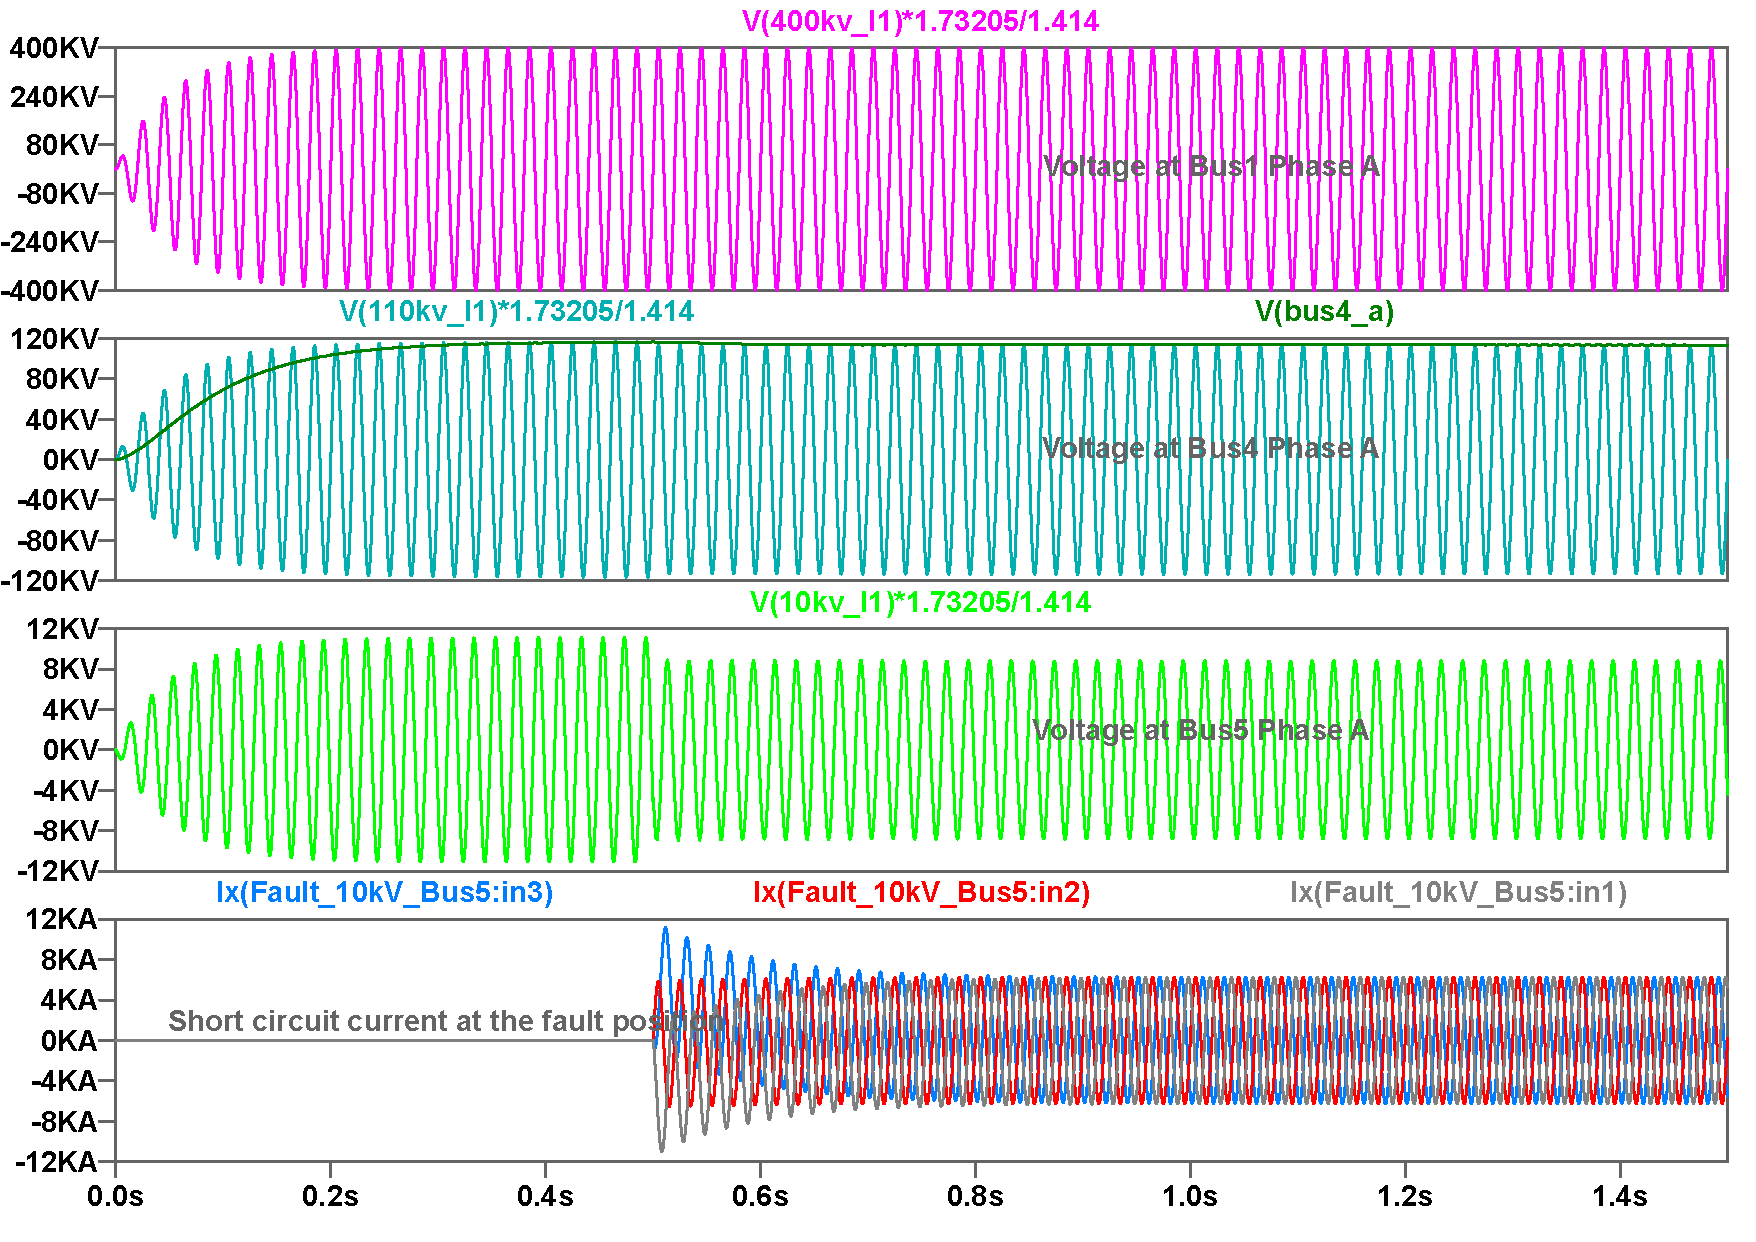
\includegraphics[width=0.9\textwidth] {figures/02_Shortcircuit in the medium voltage grid/Shortcircuit_Current_with_scr_waveform}
	\caption{Shortcircuit in the medium voltage grid with scr - waveform}
	\label{fig:figure26}
\end{figure}

\begin{figure}[H]
	\centering
	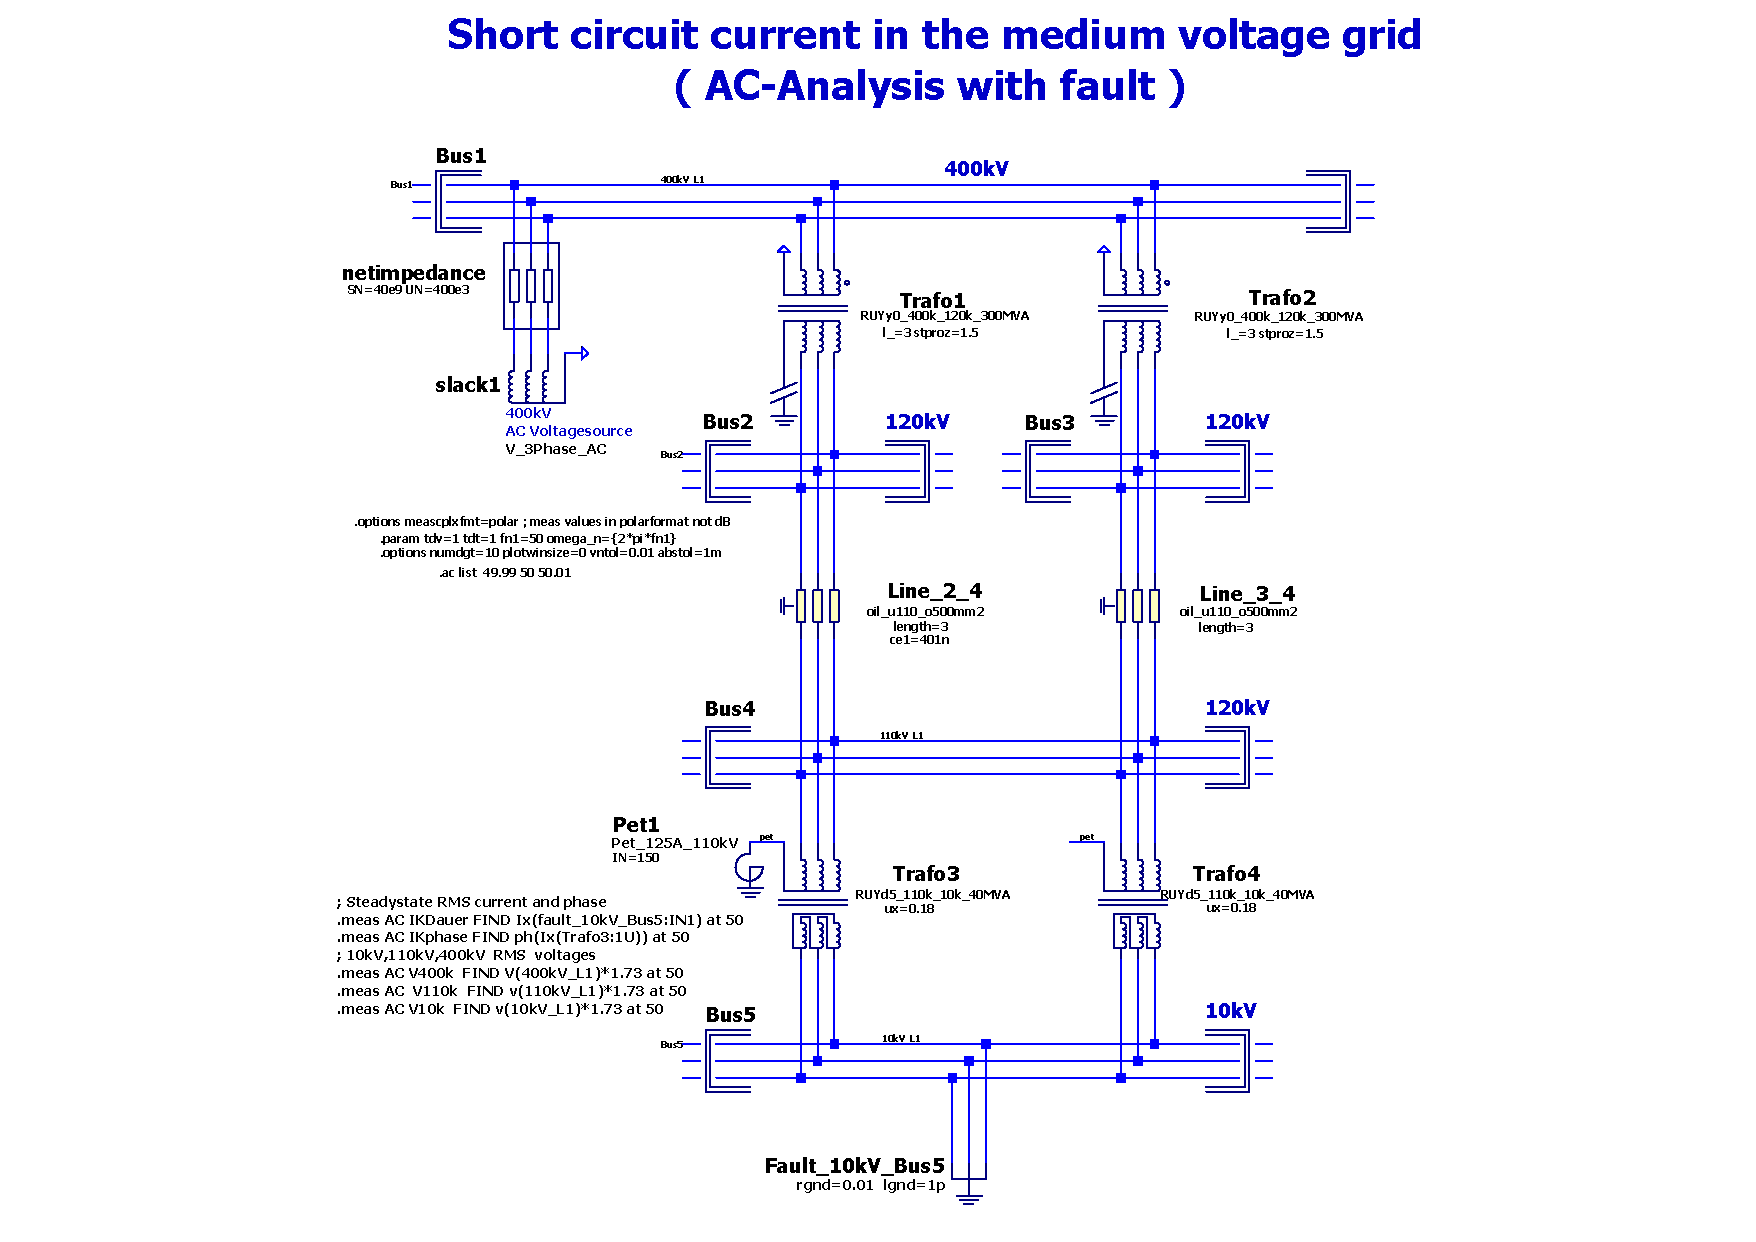
\includegraphics[width=1\textwidth] {figures/02_Shortcircuit in the medium voltage grid/Shortcircuit_Current_AC_schematic}
	\caption{Shortcircuit in the medium voltage grid AC analysis - schematic}
	\label{fig:figure27}
\end{figure}

\begin{figure}[H]
	\centering
	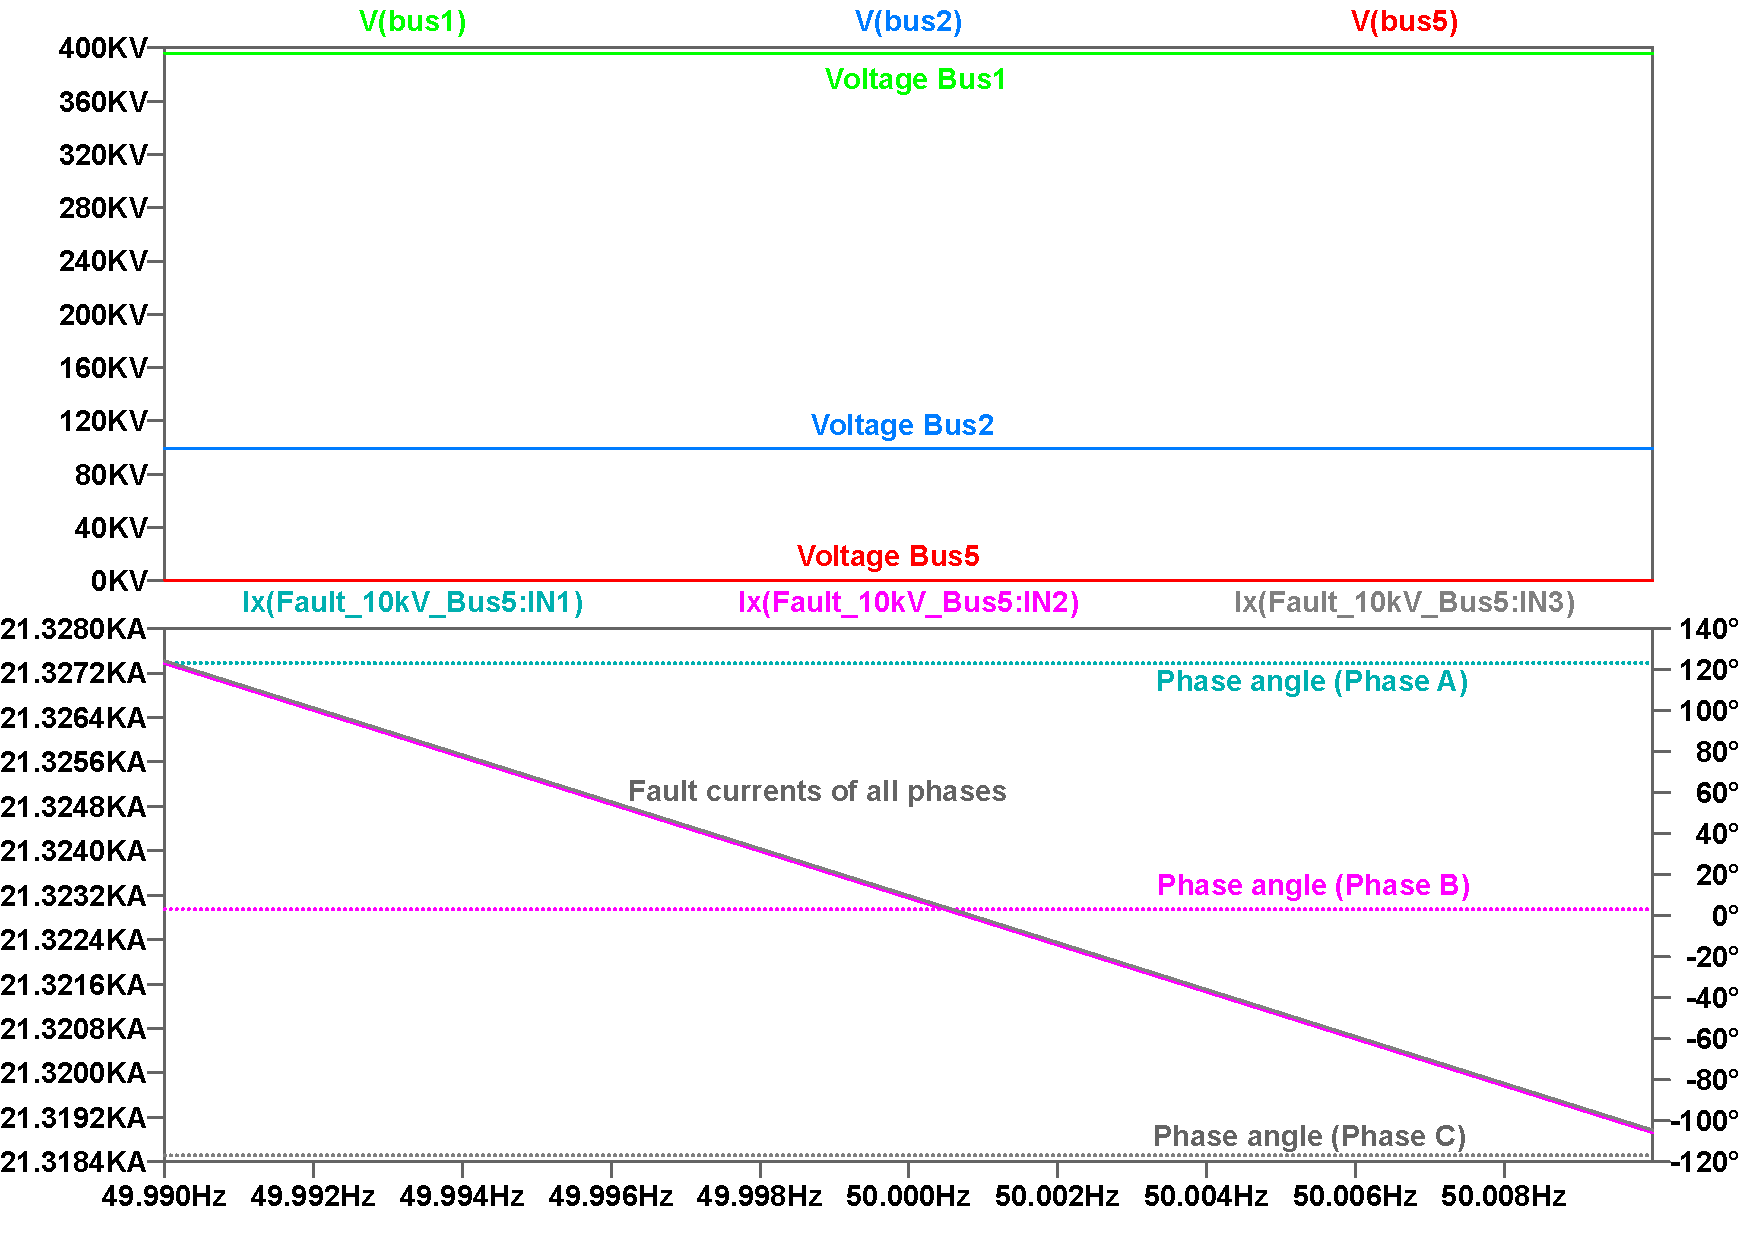
\includegraphics[width=0.9\textwidth] {figures/02_Shortcircuit in the medium voltage grid/Shortcircuit_Current_AC_waveform}
	\caption{Shortcircuit in the medium voltage grid AC analysis - waveform}
	\label{fig:figure28}
\end{figure}

\begin{chaptersummary}
Two \SI{40}{\mega\volt\ampere} medium-voltage transformers operated in
parallel produce a settled short-circuit current of approximately
\SI{22}{\kilo\ampere} RMS in the investigated network. A simple estimate based
on rated current, relative short-circuit voltage, parallel operation, and the
actual operating voltage closely reproduces this result. An initial inductive
load reduces the current slightly, whereas an additional short-circuit reactor
limits it substantially to approximately \SI{4.4}{\kilo\ampere}. The AC
analysis also demonstrates that transformer vector groups must be considered
when interpreting phase angles.
\end{chaptersummary}
